\documentclass[10pt,a4paper]{article}
\usepackage[T1]{fontenc}
\usepackage{lmodern,amsmath,amssymb,amsthm,booktabs,longtable,array,graphicx,xcolor,tikz,enumitem}
\usepackage[margin=21mm]{geometry}
\usepackage[colorlinks=true,linkcolor=blue,citecolor=blue,urlcolor=blue]{hyperref}
\usetikzlibrary{arrows.meta,positioning,calc}
\setlength{\parskip}{3pt}
\setlength{\emergencystretch}{3em}
\renewcommand{\topfraction}{0.94}
\renewcommand{\bottomfraction}{0.9}
\renewcommand{\textfraction}{0.04}
\renewcommand{\floatpagefraction}{0.85}
\setlist{nosep,leftmargin=*}
\renewcommand{\arraystretch}{1.15}
\newtheorem{proposition}{Proposition}
\newcommand{\pos}[1]{\left[#1\right]^+}
\newcommand{\norm}[1]{\left\lVert#1\right\rVert_1}
\newcommand{\algline}[3]{\node[anchor=west,font=\small] at (#2,-.48*#1) {#3};\node[anchor=east,font=\scriptsize,text=gray] at (-.15,-.48*#1) {#1}}
\title{Delay-Gated Telemetry-Aware Capacity Elasticity\\for SDN-Managed O-RAN Service Chains}
\author{}
\date{}
\begin{document}
\maketitle
\vspace{-12mm}
\begin{abstract}
Delayed observations and queued resource commands can make elastic provisioning
more expensive and less timely than fixed capacity. This paper studies that
interaction in a reproducible, O-RAN-motivated three-stage service-chain model.
A telemetry-aware controller projects reported queues using its applied-action
ledger and pending commands, then enumerates a finite capacity-and-share grid.
A deployment gate selects a separately calibrated fixed profile when configured
actuation delay reaches the shorter class deadline. An evaluation frozen after
development executes 800 policy runs across eight settings and twenty fresh seeds.
At ten-slot actuation delay, the gated policy reduces mean incremental resource
cost by @@SAVINGS@@\% in stressed settings relative to calibrated fixed capacity.
@@ABSTRACT_MISS@@ At long delays, the ungated predictor deteriorates, while the
gated policy is pathwise identical to its fixed fallback by construction.
The analysis establishes causality, conservation and finite-grid optimality for
the decision surrogate, not stochastic deadline guarantees. Paired uncertainty,
component ablations and negative results delineate when elasticity is useful.
The results concern an abstract packet-service simulator, not a physical-layer
or interoperable O-RAN implementation.
\end{abstract}
\noindent\textbf{Keywords:} Open RAN, software-defined networking, resource orchestration,
delayed telemetry, delayed actuation, queue prediction, reproducible simulation.

\section{Introduction}
Open Radio Access Network (O-RAN) makes network control and orchestration an
important part of radio-access-system design \cite{polese}. Software-defined
networking (SDN) separates programmable control from forwarding functions
\cite{sdn}, while virtualization changes how radio and computing resources are
managed \cite{ecosystem}. A practical consequence is that a resource decision
need not take effect at the instant at which the relevant queue is measured.
The controller may receive an old report, issue a command based on it, and then
observe another report before that command becomes active. Treating this sequence
as instantaneous obscures the difference between required and already-requested
capacity.

Information age formalizes the distinction between a report's delivery time and
the time represented by its contents \cite{age}. Networked control likewise
recognizes sensing and actuation delays as part of the closed-loop system
\cite{networked}. Predictive control can explicitly account for future action
effects, but its stability and optimality properties depend on the model and
constraints used \cite{mpc}. Consequently, adding a forecast to a queue heuristic
does not establish a reliability guarantee. In particular, a predictor based on
old service rates may continue requesting expansion that is already in transit.
Conversely, an optimistic projection may release capacity before a burst has
cleared.

The question considered here is deliberately narrower than full O-RAN resource
optimization: \emph{how do an action-aware queue projection, a bounded dispersion
horizon and a delay-based deployment gate affect the cost--deadline trade-off
under equal telemetry budgets?} The system contains two packet classes and three
serial service stages. The stage interpretation is access, transport and compute,
but each uses the same abstract packet-service unit. No radio propagation,
physical resource block allocation or measured processor service curve is implied.

The contributions are as follows.
\begin{enumerate}
\item A causal controller uses asynchronously timestamped reports, an applied-action
ledger and immutable pending commands to project workload at command activation.
Its finite-grid decision separates surrogate feasibility from paid capacity cost.
\item A deployment policy gates that controller by the configured actuation delay.
The fallback is selected independently by calibration, and its equivalence to the
reference is established explicitly rather than presented as a novel safety guarantee.
\item A frozen comparison includes 800 executed runs, paired seeds, both classes,
bounded-margin and ungated ablations, and long-delay failures. The evaluation
distinguishes improvement over a legacy heuristic from improvement over fixed capacity.
\item An executable event contract, conservation checks, causality tests and
independent packet replay connect the mathematical model to the reported outputs.
\end{enumerate}
The intended contribution is a controlled computational study of delayed
elasticity, not a claim that forecasting, O-RAN orchestration or policy fallback
is new in isolation. The remainder positions the model against prior work,
defines the controller and its limited formal properties, and evaluates its
cost and deadline outcomes.

\section{Related Work and Positioning}
\subsection{Orchestration and resource coupling}
OrchestRAN selects intelligence algorithms and execution locations for specified
network objectives \cite{orchestr}. OREO examines orchestration and sharing of
xApp-based services \cite{oreo}. These studies concern deployment of control
intelligence, whereas the present decision changes the capacity and class
reservations of packet-serving stages. Joint cloud, fronthaul and radio
orchestration is already studied for cell-free massive multiple-input
multiple-output systems \cite{demir}. Therefore, representing three resource
domains does not itself establish novelty.

vrAIn learns coupled radio and computing allocations using an implemented
virtualized radio access network (vRAN) \cite{vrain}. Nuberu changes the distributed-unit
processing pipeline to preserve operation under computing deficits \cite{nuberu}.
Concordia predicts task execution requirements and schedules shared computing
resources against stringent processing deadlines \cite{concordia}. These systems
motivate resource coupling but also expose a limitation of abstract tandem queues:
physical radio and processor demand are not interchangeable packet counts.

Online learning for virtualized base-station allocation \cite{kalntis} and the
delay-aware, multi-timescale MAREA orchestrator \cite{marea} address richer
resource-allocation questions. MAREA's analytical delay treatment is distinct
from the dispersion heuristic used below. Proactive artificial-intelligence
and RAN workload orchestration \cite{caora} and learning-based functional-split
selection \cite{murti} further show that anticipatory allocation and reconfiguration
costs are established research directions. No published performance figure from
these studies is imported as a baseline result in this paper.

\subsection{Prediction, slicing and control interaction}
Radio-intelligence-controller resource allocation \cite{wang}, cloud-native
multivariate probabilistic forecasting \cite{kasuluru}, and online-learning
energy-efficient allocation \cite{sora} provide complementary approaches to
resource decisions. The current predictor is neither a trained multivariate
model nor an energy model. Its purpose is to isolate whether accounting for
known actions changes a simple, fully inspectable controller.

COMIX addresses interactions among O-RAN xApps \cite{comix}. That problem differs
from one controller's sequential commands but reinforces the need to distinguish
requested actions from their combined effect. Service-enabled sub-slice isolation
\cite{5erasi} and RadioSaber's channel-aware slicing with customizable schedulers
\cite{radiosaber} concern properties not captured by the two-class quota model.
In particular, borrowing unused quota here does not prove slice isolation.
EdgeRIC demonstrates the importance of control placement and timescale in an
implemented system \cite{edgeric}. This motivates explicit delay sensitivity,
without equating a synthetic slot with its real-time control cycle.

\begin{table}[htbp]\centering\small
\caption{Closest-work distinctions. This is a conceptual comparison, not a reproduced benchmark.}
\begin{tabular}{p{29mm}p{53mm}p{66mm}}\toprule
Study & Principal decision or evidence & Distinction in the present study\\\midrule
OrchestRAN, OREO & Intelligence placement and xApp orchestration & Packet capacity, not xApp deployment\\
Demir et al. & Coupled physical cloud/fronthaul/radio resources & Three homogeneous service-unit stages\\
vrAIn, Concordia & Implemented compute/radio control and deadline scheduling & No calibrated CPU or physical radio model\\
Kalntis et al. & Online-learning vBS allocation & Deterministic finite-grid heuristic, no regret result\\
MAREA & Multi-timescale delay-aware radio orchestration & Deadline proxy, not an analytical violation bound\\
Probabilistic forecasting & Data-driven predictive resource information & Fixed-history, action-ledger projection\\
EdgeRIC & Low-latency control with a real RAN stack & Configured synthetic actuation-delay experiment\\
This study & Matched traces, pending commands, ablations and fallback & Conditional cost--delay evidence with explicit failure regimes\\\bottomrule
\end{tabular}\label{tab:related}
\end{table}

\subsection{Experimental platforms and analytical boundaries}
ColO-RAN \cite{coloran}, OpenRAN Gym \cite{gym}, SCOPE \cite{scope}, and FlexRIC
\cite{flexric} support experimental programmable-RAN work. ns-O-RAN integrates
simulation with a RAN Intelligent Controller (RIC) \cite{nsoran}, while Colosseum
supports digital-twin experimentation \cite{colosseum}. The end-to-end 5G-LENA
simulator \cite{lena} and its calibration studies \cite{calibration} provide a
route toward radio-aware evaluation. These platforms were not executed in the
present experiments. Their relevance is methodological, not evidence of
interoperability for this implementation.

Queue-based stochastic optimization \cite{neely}, deterministic network calculus
\cite{netcalc}, and stochastic network calculus \cite{stochcalc} distinguish
long-run stability, worst-case delay and probabilistic guarantees. Scheduler
analyses for interleaved weighted round-robin \cite{iwrr}, deficit round-robin
\cite{drr}, and packet-level arrival constraints \cite{packetbounds} further
show that precise service assumptions matter. The controller below uses none
of those service-curve guarantees. This distinction is important because a low
surrogate score is not proof of an end-to-end packet deadline. Finally,
verification of an implemented abstraction is separate from validation against
its intended physical system \cite{sargent}.

\section{System Model and Problem Definition}
\subsection{State, service and event order}
Let $i\in\{1,2,3\}$ index stages, $s\in\{0,1\}$ index classes and
$t\in\{0,\ldots,T-1\}$ index discrete slots. A packet has a class $s$, birth
slot $b$ and absolute deadline $b+D_s-1$. A packet completed in slot $t$ has
latency $t-b+1$ and is late if that value exceeds $D_s$.
Let $Q_{is}(t)$ denote the queue at the beginning of slot $t$, before external
arrivals, and let $A_s(t)$ denote newly generated packets. Service $S_{is}(t)$
uses total integer capacity $C_i(t)=c_i(t)+e_i(t)$, comprising base capacity
$c_i$ and active paid expansion $e_i$. The implemented dynamics are
\begin{align}
 Q_{1s}(t+1)&=Q_{1s}(t)+A_s(t)-S_{1s}(t),\label{eq:q1}\\
 Q_{is}(t+1)&=Q_{is}(t)-S_{is}(t)+S_{i-1,s}(t),\quad i=2,3.\label{eq:qi}
\end{align}
Stage 1 can serve new arrivals immediately. Stages 2 and 3 serve before their
upstream neighbors, so a packet cannot traverse two stages in one slot.
Each packet requires one service unit at every stage. Class queues are first-in,
first-out (FIFO). There are no drops, retransmissions, alternate routes or
finite-buffer admission decisions.

At each slot the engine applies due commands, delivers due reports, inserts
external arrivals, requests a report and computes a command if the slot is a
control epoch, serves stages in order $3,2,1$, and updates measurement histories.
This ordering fixes otherwise consequential ambiguities at equal timestamps.
Report snapshots are taken after external arrivals and before service.
No new snapshot is visible to the controller before its configured delivery time.

\begin{figure}[htbp]\centering
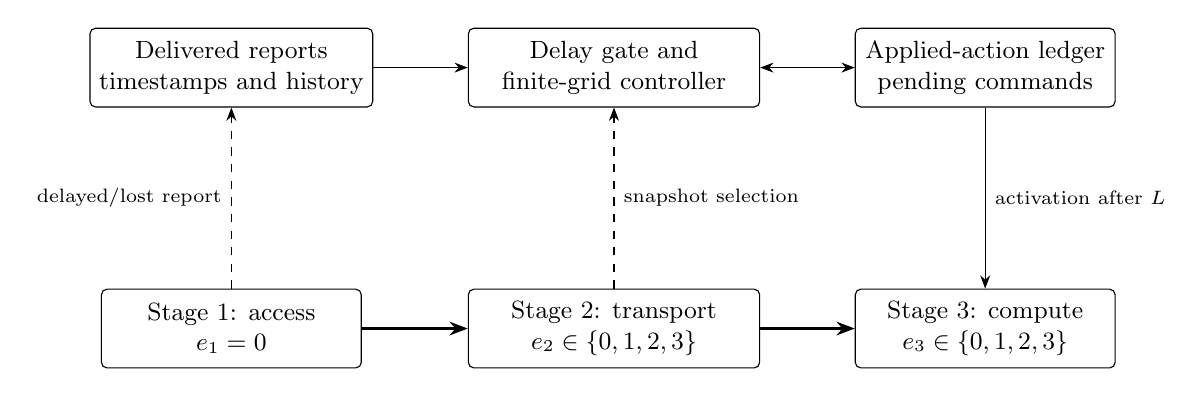
\begin{tikzpicture}[>=Stealth,box/.style={draw,rounded corners=2pt,align=center,minimum height=10mm,font=\small},node distance=11mm]
\node[box,minimum width=33mm] (r) {Delivered reports\\timestamps and history};
\node[box,right=12mm of r,minimum width=37mm] (ctrl) {Delay gate and\\finite-grid controller};
\node[box,right=12mm of ctrl,minimum width=33mm] (a) {Applied-action ledger\\pending commands};
\node[box,below=23mm of r,minimum width=33mm] (s1) {Stage 1: access\\$e_1=0$};
\node[box,below=23mm of ctrl,minimum width=37mm] (s2) {Stage 2: transport\\$e_2\in\{0,1,2,3\}$};
\node[box,below=23mm of a,minimum width=33mm] (s3) {Stage 3: compute\\$e_3\in\{0,1,2,3\}$};
\draw[->] (r)--(ctrl);
\draw[<->] (ctrl)--(a);
\draw[->,thick] (s1)--(s2);
\draw[->,thick] (s2)--(s3);
\draw[->,dashed] (s1)--node[left,font=\scriptsize]{delayed/lost report}(r);
\draw[->,dashed] (s2.north)--node[right,font=\scriptsize]{snapshot selection}(ctrl.south);
\draw[->] (a.south)--node[right,font=\scriptsize]{activation after $L$}(s3.north);
\end{tikzpicture}
\caption{Implemented abstract service chain and information paths. All stages can
report and receive class-share commands. Only stages 2 and 3 can expand capacity.
The domain labels are an O-RAN motivation, not implemented protocol entities.}
\label{fig:architecture}
\end{figure}

\begin{table}[htbp]\centering\small
\caption{Notation and units. All capacities and workloads are abstract.}
\begin{tabular}{p{32mm}p{117mm}}\toprule
Symbol & Definition\\\midrule
$Q_{is},A_s,S_{is}$ & Queue, external arrivals and service counts, in packets\\
$c_i,e_i,C_i$ & Base, expansion and total capacity, in packets per slot\\
$D_s,b,T$ & Class deadline, birth slot and run length, in slots\\
$\tau_i,\Delta_i$ & Timestamp of latest delivered stage report and its age $t-\tau_i$\\
$\bar a_{is},\bar\mu_{is},v_{is}$ & Historical mean ingress, mean service and variance of net ingress\\
$h,W,R,L,p$ & Control interval, history window, report delay, activation delay and report loss probability\\
$\alpha,k,\mathcal X$ & Class-0 share, share-grid index and candidate decision set\\
$\mathcal L,\mathcal P$ & Applied-action ledger and pending-command list\\
$\widehat q_{is},d_{is},\rho_s$ & Projected pre-service queue, demand proxy and normalized delay score\\
$J,V_s$ & Full-run incremental cost and cohort deadline-miss fraction\\\bottomrule
\end{tabular}
\end{table}

\subsection{Reservations and local borrowing}
For weights $(\alpha,1-\alpha)$, integer reserved service
$g_{is}(C_i,\alpha)$ is obtained by flooring proportional quotas and assigning
the remainder to the largest fractional part, with deterministic class-index
tie breaking. Thus $\sum_s g_{is}=C_i$.
The local scheduler first reserves
\begin{equation}
 u_{is}=\min\{B_{is},g_{is}\},\qquad
 B_{1s}=Q_{1s}+A_s,\quad B_{is}=Q_{is}\ (i>1).
\end{equation}
Remaining units are borrowed by the eligible class whose next packet has the
earliest absolute deadline, with class-index ties. This is deadline-based
borrowing after reservations, not unrestricted earliest-deadline-first service.
It ensures $\sum_s S_{is}=\min\{C_i,\sum_s B_{is}\}$.

\subsection{Telemetry and immutable commands}
Every $h=5$ slots, one stage is selected for a report. Its payload is
\begin{equation}
 r_i=(q_i,\bar a_i,\bar\mu_i,v_i,\bar c_i,\tau_i),
\end{equation}
where $q_i$ is the pre-service queue, $\bar c_i$ is the base capacity at the
snapshot, and the rate statistics use the preceding $W=20$ slots.
Specifically, $v_{is}$ is the population variance of stage ingress minus service
over that window. Empty histories use fixed initialization values listed in the
experiment setup. Each request is independently lost with probability $p$ or
delivered after $R$ slots. A report older than the stored timestamp is discarded.

The common risk-based report selector uses
\begin{align}
 \widetilde q_{is}(t)&=\pos{q_{is}+\Delta_i(\bar a_{is}-\bar\mu_{is})},\\
 z_i(t)&=\sum_s\frac{\sqrt{\Delta_i v_{is}+1}}{D_s}
 \left(1+\frac{\widetilde q_{is}(t)}{\max(1,\bar c_i)}\right)+0.01\Delta_i.
\end{align}
The stage with greatest $z_i$ is selected, breaking ties by stage index.
The final age term is a heuristic priority term, not a bounded-starvation proof.
Different methods may select different stages even though their request counts
and request-index loss flags are identical.

A decision at time $t$ creates an immutable command $(t+L,x,w)$ containing an
expansion vector and stage-wise class weights. All due commands execute. There
is no cancellation, acknowledgment loss, out-of-order actuation or supersession.
Since $L$ is fixed within each run, chronological decision order is preserved.
Initial fixed capacity is preprovisioned, whereas elastic methods start with
zero expansion. Fixed methods still update class shares through delayed commands.

\begin{figure}[htbp]\centering
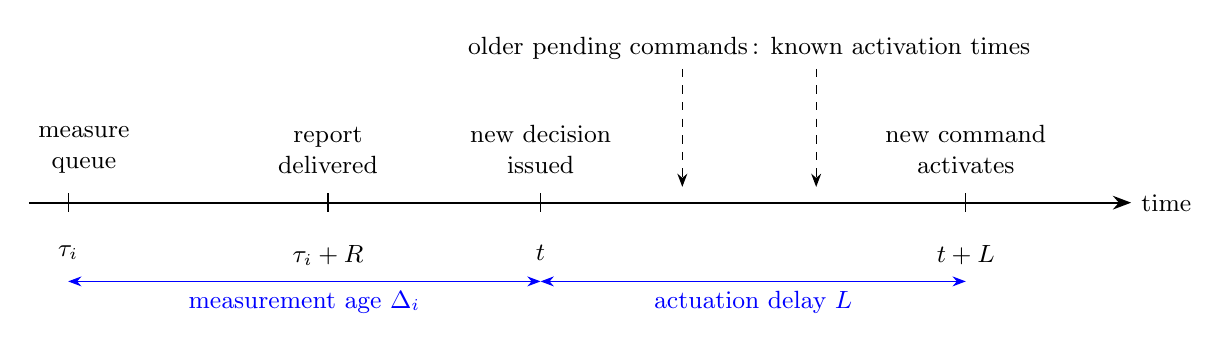
\begin{tikzpicture}[>=Stealth,x=1cm,y=1cm,font=\small]
\draw[->,thick] (0,0)--(14,0) node[right] {time};
\foreach \x/\lab in {0.5/{$\tau_i$},3.8/{$\tau_i+R$},6.5/{$t$},11.9/{$t+L$}}{
 \draw (\x,.12)--(\x,-.12) node[below=3mm] {\lab};}
\node[above,align=center] at (.7,.25) {measure\\queue};
\node[above,align=center] at (3.8,.25) {report\\delivered};
\node[above,align=center] at (6.5,.25) {new decision\\issued};
\node[above,align=center] at (11.9,.25) {new command\\activates};
\draw[<->,blue] (.5,-1)--node[below] {measurement age $\Delta_i$}(6.5,-1);
\draw[<->,blue] (6.5,-1)--node[below] {actuation delay $L$}(11.9,-1);
\draw[->,dashed] (8.3,1.7)--(8.3,.2);
\draw[->,dashed] (10,1.7)--(10,.2);
\node[above,align=center] at (9.15,1.7) {older pending commands\,: known activation times};
\end{tikzpicture}
\caption{Projection spans report age and actuation delay. Commands already pending
can change service before the new command activates. The new command itself is
excluded when predicting the pre-service state at $t+L$.}
\label{fig:timeline}
\end{figure}

\subsection{Objective and measured reliability}
The incremental resource objective is
\begin{equation}
 J=\sum_{t=0}^{T-1}\sum_i e_i(t)
 +\kappa\sum_{t=1}^{T-1}\norm{e(t)-e(t-1)},\qquad\kappa=0.25.\label{eq:cost}
\end{equation}
It includes warm-up and tail capacity, charges actual expansion changes, and
excludes base-resource costs. Initial provisioning incurs no switching charge.
Units are abstract resource cost units, not money, energy or measured power.

For the measured birth cohort $\mathcal C_s$, let $N_s=|\mathcal C_s|$ and let
$\ell_p$ be completion latency. The miss fraction is
\begin{equation}
 V_s=\frac{\#\{p\in\mathcal C_s:\ell_p>D_s\}
 +\#\{p\in\mathcal C_s:p\text{ unfinished at run end}\}}{\max(1,N_s)}.\label{eq:miss}
\end{equation}
The tail extends beyond all measured deadlines, so unfinished cohort packets
are known misses rather than right-censored successes. Background arrivals
continue during that tail. Calibration uses a 1\% mean-miss criterion for each
class, but this finite-sample selection rule is not a chance constraint.

The ideal design problem minimizes expected $J$ under classwise reliability
requirements using only available information. The implemented method does not
solve that stochastic control problem. It solves the per-decision surrogate
defined next, and its actual reliability is measured separately.

\section{Delay-Gated Action-Aware Controller}
\subsection{Projection from the action ledger}
At decision time $t$, the ledger $\mathcal L(u)$ records the expansion and weights
actually applied at slots $u\le t$. The list $\mathcal P(t)$ contains commands
already issued but not yet activated. Their deterministic activation times
define a known action trajectory up to $t+L-1$. This uses no future exogenous
arrivals or capacity realizations.

For each stage, initialize $\widehat q_i(\tau_i)=q_i$ and hold its latest
reported base capacity and mean ingress constant. The fluid recurrence is
\begin{equation}
 \widehat q_{is}(u+1)=\pos{\widehat q_{is}(u)-F_s(\widehat q_i(u),w_i(u),
 \bar c_i+e_i(u))}+\bar a_{is},
 \quad u=\tau_i,\ldots,t+L-1.\label{eq:project}
\end{equation}
The fluid service operator $F$ first applies integer reservations, limited by
the real-valued projected workload, and assigns spare units in descending order
of normalized residual workload $(\widehat q_{is}-u_{is})/D_s$. Ties use the class
index. The projection does not contain packet ages, so this borrowing rule is
only an approximation to the packet scheduler.

Each stage is projected independently using its last reported ingress.
Projected upstream departures are not fed into the downstream forecast.
This avoids pretending that asynchronously observed queues constitute a
consistent instantaneous network state, but it also omits propagation of
future upstream actions. The ledger is action-aware, not a perfect network
predictor. The state at $t+L$ is pre-service and therefore excludes the effect
of the new candidate command on that slot's service.

\begin{figure}[htbp]\centering
\begin{minipage}{.96\linewidth}
\textbf{Algorithm 1. Applied-action and pending-command projection}\par\smallskip\hrule\smallskip
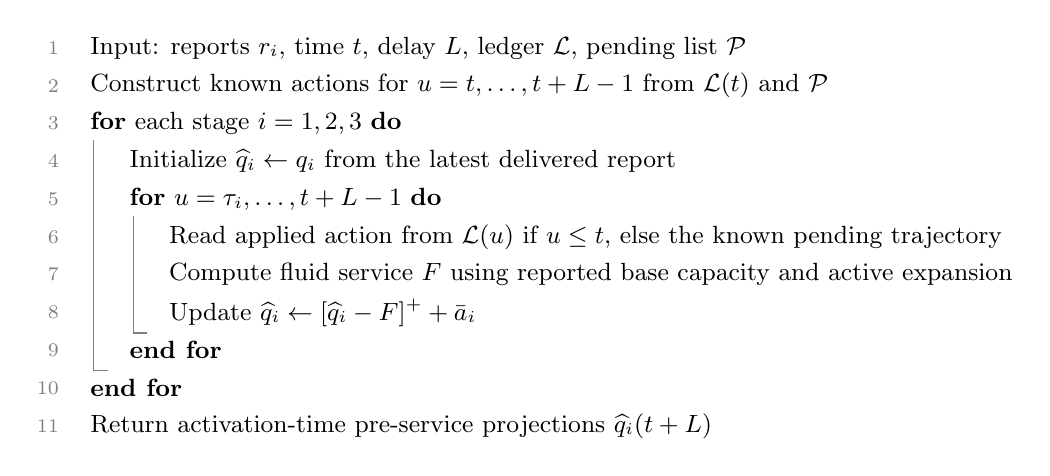
\begin{tikzpicture}[x=1cm,y=1cm]
\algline{1}{0}{Input: reports $r_i$, time $t$, delay $L$, ledger $\mathcal L$, pending list $\mathcal P$};
\algline{2}{0}{Construct known actions for $u=t,\ldots,t+L-1$ from $\mathcal L(t)$ and $\mathcal P$};
\algline{3}{0}{\textbf{for} each stage $i=1,2,3$ \textbf{do}};
\algline{4}{.5}{Initialize $\widehat q_i\leftarrow q_i$ from the latest delivered report};
\algline{5}{.5}{\textbf{for} $u=\tau_i,\ldots,t+L-1$ \textbf{do}};
\algline{6}{1}{Read applied action from $\mathcal L(u)$ if $u\le t$, else the known pending trajectory};
\algline{7}{1}{Compute fluid service $F$ using reported base capacity and active expansion};
\algline{8}{1}{Update $\widehat q_i\leftarrow [\widehat q_i-F]^++\bar a_i$};
\algline{9}{.5}{\textbf{end for}};
\algline{10}{0}{\textbf{end for}};
\algline{11}{0}{Return activation-time pre-service projections $\widehat q_i(t+L)$};
\draw[gray] (.17,-1.65)--(.17,-4.58)--(.35,-4.58);
\draw[gray] (.67,-2.61)--(.67,-4.1)--(.85,-4.1);
\end{tikzpicture}\hrule
\end{minipage}
\end{figure}

\subsection{Finite-grid surrogate}
The bounded-horizon demand proxy is
\begin{equation}
 d_{is}=\widehat q_{is}(t+L)+h\bar a_{is}+\sqrt{h v_{is}}+1.\label{eq:demand}
\end{equation}
The square-root term is a dispersion heuristic evaluated over one control
interval. It is not a confidence bound on the longer queue-projection horizon.
The additive one-packet term is a fixed conservative offset. Both are explicit
design choices, not parameters inferred from O-RAN measurements.

The decision grid contains
\begin{equation}
 \mathcal X=\{(x,\alpha):x=(0,x_2,x_3),\ x_2,x_3\in\{0,1,2,3\},
 \ \alpha=k/20,\ k=1,\ldots,19\},\quad |\mathcal X|=304.
\end{equation}
The same share is applied at all stages. With reported base capacities,
candidate integer reservations yield
\begin{align}
 \rho_s(x,\alpha)&=\frac1{D_s}\sum_i
 \frac{d_{is}}{\max\{10^{-3},g_{is}(\bar c_i+x_i,\alpha)\}},\\
 r(x,\alpha)&=\max_s\rho_s(x,\alpha),\\
 c(x)&=\sum_i x_i+\kappa\norm{x-x^{\mathrm{req}}_{\mathrm{prev}}}.\label{eq:proxycost}
\end{align}
The small denominator floor defines a finite penalty for zero reservations,
not guaranteed fractional service. The cost proxy compares with the previous
\emph{requested} expansion. It differs intentionally from the realized cost in
\eqref{eq:cost}, which uses actual activation changes.

Candidates are ranked lexicographically by
\begin{equation}
 \sigma(x,\alpha)=
 \begin{cases}
 (0,c,r,\sum_s\rho_s,k), & r\le1,\\
 (1,r,c,\sum_s\rho_s,k), & r>1.
 \end{cases}\label{eq:ranking}
\end{equation}
The minimum is selected, retaining the earliest enumerated expansion on any
remaining tie. Feasible candidates prioritize cost. When none is feasible,
the least worst-class ratio is selected. No claim of feasibility is made for
the realized packet system from this surrogate decision.

\subsection{Deployment gate and comparators}
Let $x^{\mathrm{fix}}$ be the separately calibrated fixed profile for the
scenario, and define $G=\min_s D_s=15$ slots. The proposed policy is
\begin{equation}
 \pi_{\mathrm{gate}}(L)=
 \begin{cases}
 \pi_{\mathrm{pipe}}, & L<G,\\
 \pi_{\mathrm{fix}}, & L\ge G.
 \end{cases}\label{eq:gate}
\end{equation}
This choice is made before the run using its configured constant delay. The
fallback starts preprovisioned and retains the fixed reference's class-share
controller. It is not an online switch that instantly acquires capacity after
latency rises. The threshold is an interpretable development choice, not a
derived stability boundary.

The legacy comparator replaces the action projection with
$[q_{is}+(\Delta_i+L)(\bar a_{is}-\bar\mu_{is})]^+$ and uses dispersion
$\sqrt{(\Delta_i+L)v_{is}}$. The margin-only ablation retains that legacy drift
projection but uses $\sqrt{h v_{is}}$. The ungated pipeline uses
\eqref{eq:project}--\eqref{eq:ranking} at every delay. These are inspectable
internal comparators, not reproductions of the published algorithms in
Table~\ref{tab:related}.

\begin{figure}[htbp]\centering
\begin{minipage}{.96\linewidth}
\textbf{Algorithm 2. Delay-gated deployment and elastic decision}\par\smallskip\hrule\smallskip
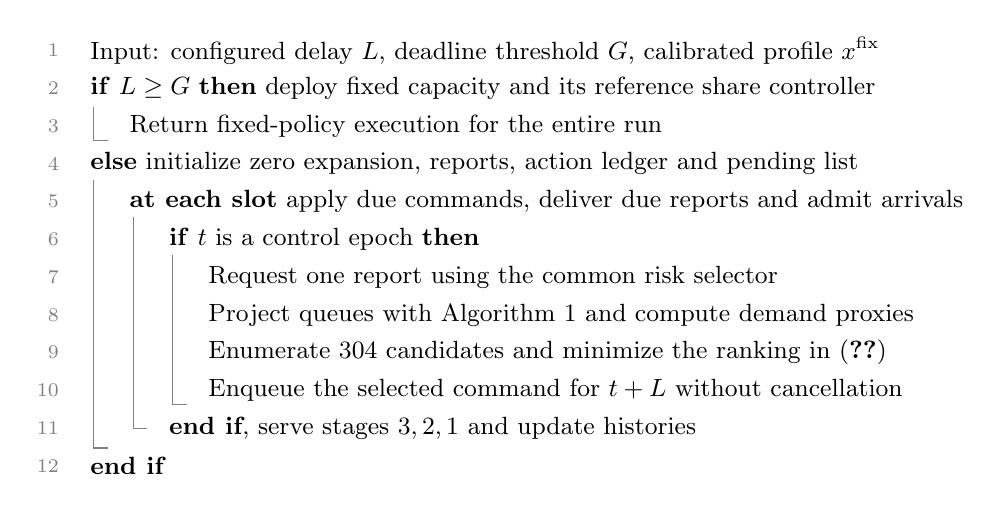
\begin{tikzpicture}[x=1cm,y=1cm]
\algline{1}{0}{Input: configured delay $L$, deadline threshold $G$, calibrated profile $x^{\mathrm{fix}}$};
\algline{2}{0}{\textbf{if} $L\ge G$ \textbf{then} deploy fixed capacity and its reference share controller};
\algline{3}{.5}{Return fixed-policy execution for the entire run};
\algline{4}{0}{\textbf{else} initialize zero expansion, reports, action ledger and pending list};
\algline{5}{.5}{\textbf{at each slot} apply due commands, deliver due reports and admit arrivals};
\algline{6}{1}{\textbf{if} $t$ is a control epoch \textbf{then}};
\algline{7}{1.5}{Request one report using the common risk selector};
\algline{8}{1.5}{Project queues with Algorithm 1 and compute demand proxies};
\algline{9}{1.5}{Enumerate $304$ candidates and minimize the ranking in (\ref{eq:ranking})};
\algline{10}{1.5}{Enqueue the selected command for $t+L$ without cancellation};
\algline{11}{1}{\textbf{end if}, serve stages $3,2,1$ and update histories};
\algline{12}{0}{\textbf{end if}};
\draw[gray] (.17,-1.2)--(.17,-1.62)--(.35,-1.62);
\draw[gray] (.17,-2.12)--(.17,-5.53)--(.35,-5.53);
\draw[gray] (.67,-2.6)--(.67,-5.28)--(.85,-5.28);
\draw[gray] (1.17,-3.08)--(1.17,-4.98)--(1.35,-4.98);
\end{tikzpicture}\hrule
\end{minipage}
\end{figure}

\section{Formal Properties and Limits}
\begin{proposition}[Causality]
For fixed configuration and initialization, every elastic decision at time $t$
is a function only of reports delivered by $t$, commands already issued and
their known activation times. It is independent of unobserved future traffic
and base-capacity realizations.
\end{proposition}
\begin{proof}
The report selector reads only stored payloads and their timestamps. The ledger
contains previously applied commands. The pending list contains commands issued
at earlier epochs. Equation~\eqref{eq:project} uses these actions and holds
reported base capacity and ingress fixed. The demand and ranking equations are
deterministic functions of that projection. Induction over decision epochs
therefore excludes future exogenous trace entries. A future-suffix perturbation
test additionally checks this property in the executable implementation.
\end{proof}

\begin{proposition}[Conservation and service bounds]
For every slot, all queues remain nonnegative, stage service does not exceed
available capacity, and the total number of generated packets equals completed
packets plus packets remaining in the chain. Completed latency is at least
three slots.
\end{proposition}
\begin{proof}
Reservations are limited by available queue contents. Borrowing only selects a
class with a remaining packet and stops at capacity, proving nonnegativity and
the service bound. Summing \eqref{eq:q1}--\eqref{eq:qi} cancels each internal
transfer, leaving external arrivals minus final-stage completions. Induction
from empty queues proves conservation. Reverse stage order prevents a packet
from receiving two stages of service in one slot, giving the latency bound.
\end{proof}

\begin{proposition}[Finite-grid decision optimality]
The enumerator returns a minimum of \eqref{eq:ranking} on $\mathcal X$.
If any surrogate-feasible candidate exists, the result is surrogate-feasible
and has minimum proxy cost among all such candidates.
\end{proposition}
\begin{proof}
All sixteen expansion vectors and nineteen share values are visited. The
running incumbent changes only for a strictly smaller lexicographic score.
After the last candidate it is a minimum over the complete finite set. The
leading score component ranks every feasible candidate ahead of every infeasible
candidate, and cost is the first varying component within the feasible subset.
This establishes the stated result, not global stochastic-control optimality.
\end{proof}

\begin{proposition}[Pathwise fallback equivalence]
For $L\ge G$, the gated policy and calibrated fixed reference have identical
packet trajectories and metrics under the same exogenous trace and report-loss
sequence.
\end{proposition}
\begin{proof}
Both execute the same reference procedure with the same initial preprovisioned
capacity, reports, weights, configuration and randomness. Their first-slot
states are equal. If states and pending events are equal before a slot, the
deterministic event contract produces equal updated states and events.
Induction establishes identical service and completion trajectories and hence
identical $V_s$ and $J$.
\end{proof}
This result transfers the reference's behavior, including any misses. It does
not improve or certify the reference's reliability.

\subsection{Capacity obstruction and computational cost}
A necessary condition for all packets in any cohort to meet their deadlines
is that each stage has enough cumulative service opportunities within the
union of their allowable residence intervals. In particular, if a cohort born
in $[a,b]$ has $N$ packets and maximum deadline $D_{\max}$, then
\begin{equation}
 N\le\sum_{t=a}^{b+D_{\max}-1} C_i(t)\qquad\text{for every stage }i.\label{eq:cut}
\end{equation}
Every such packet must consume one unit at every stage within that interval.
Violation of \eqref{eq:cut} therefore precludes universal deadline satisfaction.
The condition is loose and not sufficient because it ignores class deadlines,
competing packets, stage precedence and service timing.

With two classes and three stages fixed, projection work scales with
$\sum_i(\Delta_i+L)$. The grid requires 304 candidate scores, with reusable
stage/share calculations. In the general $m$-stage extension with $E+1$
expansion levels at each expandable stage and $K$ shares, exhaustive selection
scales as $O(K(E+1)^{m-1}mS)$ for $S$ classes. Thus the small present grid is
not evidence of scalability to many independent resource domains. The reference
implementation retains a full applied-action ledger. A production implementation
could discard entries older than the oldest stored report, subject to its report
delivery contract. No wall-clock real-time feasibility claim is made.

\section{Experimental Method}
\subsection{Synthetic workload and calibration}
All numerical parameters are synthetic design choices. A run contains 3340
slots, including 300 warm-up slots, a measured birth cohort spanning 3000 slots,
and a 40-slot tail. A convenient 20 ms per slot mapping gives deadlines of
300 and 800 ms, not ultra-reliable low-latency communication targets.
The fundamental reported delay unit remains the slot.

\begin{table}[htbp]\centering\small
\caption{Fixed experiment parameters. Poisson draws and capacity fluctuations are exogenous.}
\begin{tabular}{p{59mm}p{90mm}}\toprule
Parameter & Value\\\midrule
Classes, stages, deadlines & $2$, $3$, $(D_0,D_1)=(15,40)$ slots\\
Nominal Poisson arrival means & $(0.9,2.1)$ packets per slot\\
Burst arrival means & $(1.8,3.8)$ during $t\bmod600\in[180,290)$\\
Base capacity & $5+\xi$, with $\xi$ sampled from $(-1,0,0,1)$\\
Stressed-stage capacity & $3$ during $t\bmod600\in[170,310)$\\
Control interval and history & $h=5$ and $W=20$ slots\\
Report delay/loss & $(R,p)=(3,0.05)$ or $(9,0.15)$\\
Actuation delays & $L\in\{1,10,25,50,100\}$ across specified cases\\
Expansion and share grid & $(0,x_2,x_3)$, $x_i\in\{0,1,2,3\}$ and $\alpha=k/20$\\
Initial reported queues/capacity & $(0,0)$ and $5$ at each stage\\
Initial reported means/variance & Ingress $(0.9,2.1)$, service $(2.5,2.5)$, variance $(1,1)$\\
Initial weights & Equal class weights at each stage\\
Switching weight and gate & $\kappa=0.25$, $G=15$ slots\\\bottomrule
\end{tabular}
\end{table}

The nominal case uses nominal arrivals and no capacity-stress window.
Transport and compute cases introduce burst arrivals and stress stage 2 or 3,
respectively. The delayed/lost-report case uses transport stress with $(R,p)=(9,0.15)$.
Five independent calibration seeds, 4000--4004, selected the cheapest of all
sixteen fixed profiles with both class mean miss fractions at most 1\%.
The selected profiles were $(x_2,x_3)=(0,0)$ for nominal, $(2,0)$ for transport
and delayed/lost reports, and $(0,2)$ for compute. They were frozen before the
current controller development and not retuned for the evaluation seeds or
the longer activation delays. A fixed profile is therefore a strong calibrated
comparator for its scenario, not an oracle that sees the test trace.

\subsection{Development, locked evaluation and equal budgets}
Development used seeds 8000--8004 at $L=10$ and $100$ for four variants, giving
40 runs. It revealed severe long-delay misses for the ungated action-aware
projection and informed the deployment gate. These development results are
retained in the reproducibility package and excluded from confirmatory summaries.
The gate, fixed profiles, margin, objective and evaluation matrix were recorded
before using fresh seeds 9000--9019.

The locked matrix contains the four original scenarios at $L=10$ and ordinary
transport stress at $L=1,25,50,100$. Each of these eight settings runs five
methods on twenty seeds, producing $8\times5\times20=800$ executions. Gated
and pipeline policies coincide below the gate, while gated and fixed coincide
above it. These duplicated policy runs verify equivalence but do not increase
the number of independent seeds.

Within a setting, every method receives the same arrivals and base capacities,
verified by trace hashes. The same seeded request-index loss flags are used,
and each method requests one report every five slots. Stage selections can
differ, and consequently identical delivered-report counts do not mean identical
report contents. The paired design controls exogenous variation without giving
any controller privileged queue information.

\subsection{Uncertainty, testing and verification}
Reported metrics average the twenty seed-level miss fractions and costs, rather
than pooling all packets across seeds. Percentile bootstrap intervals use 10,000
seed resamples \cite{efron}. Differences use paired resampling of seed-level
differences. The bootstrap unit is the independent seed, not an individual
correlated packet. All-zero samples can yield a zero-width interval and do not
establish zero true violation probability.

Exact two-sided sign tests exclude exact ties. A Holm adjustment \cite{holm}
controls the declared family of 48 tests comprising eight settings, two
comparators (legacy and fixed), and three endpoints (two miss fractions and
cost). The sign test concerns the direction of paired differences, not their
mean. Neither a nonsignificant test nor an interval spanning zero establishes
equivalence or reliability noninferiority. Percentage-point differences are
used for miss rates to avoid unstable relative changes near zero.

Verification comprises @@TESTCOUNT@@ unit-test methods, historical-regression
checks, an independently implemented packet replay, an uncached enumeration
reference, and reconciliation of new result records. The independent replay
checks the packet engine against recorded actions, not the predictive model's
physical validity. Dedicated tests exercise pending commands, activation-time
boundaries, future-data exclusion, and gated-policy equivalence. All numerical
tables and result plots below are generated directly from saved execution
records, not manually entered performance targets.

\section{Results}
\subsection{Primary settings at ten-slot actuation delay}
Table~\ref{tab:primary} reports all five methods. In this regime, the deployment
gate selects the pipeline method, so its identical rows are expected. The
nominal case has zero fixed expansion cost, making percentage savings relative
to that reference undefined. Any elastic activation there is an additional
cost, not an efficiency gain.

@@PRIMARY_TABLE@@

Across the three stressed settings, mean incremental cost savings of the gated
policy relative to fixed capacity are @@SAVINGS@@\%.
@@PRIMARY_NARRATIVE@@ The conclusion is therefore a cost--deadline trade-off
within the evaluated workload family, not a uniform ordering of policies.
The scatter plot in Fig.~\ref{fig:tradeoff} makes that trade-off visible without
combining cost and misses into a post hoc scalar performance score.

\begin{figure}[htbp]\centering
\includegraphics[width=.96\linewidth]{primary.pdf}
\caption{Primary comparison at $L=10$. Error bars are seed-bootstrap 95\%
intervals. Gated equals pipeline in these settings. Cost is incremental and
does not include the base service infrastructure.}\label{fig:primary}
\end{figure}

\subsection{Ablation and prediction limits}
The margin-only method changes the dispersion horizon without adding an action
ledger. Comparing it with legacy isolates that change. Comparing pipeline with
margin-only then assesses the action-aware projection conditional on the same
bounded margin. This sequential ablation does not identify every possible
interaction. A ledger-only variant was examined during development but is not
part of the five-method locked matrix.

At long delay the full ungated predictor remains vulnerable. A known action
trajectory does not reveal future bursts or future base-capacity changes, and
independent stage projection does not preserve dynamic coupling between stage
departures and downstream ingress. The bounded margin also stops growing with
the projection horizon. Consequently, projection awareness alone cannot be
interpreted as robustness to arbitrary sensing and actuation delay.

\begin{figure}[htbp]\centering
\includegraphics[width=.96\linewidth]{tradeoff.pdf}
\caption{Cost--deadline outcomes in the three stressed primary settings. Each
marker is a twenty-seed mean, not a Pareto-optimality certificate. The two
rows retain both classes rather than hiding the class with the worse trade-off.}
\label{fig:tradeoff}
\end{figure}

\subsection{Activation-delay sensitivity and gated fallback}
Figure~\ref{fig:delay} includes transport stress at all five evaluated actuation
delays. At $L\ge15$, the gated implementation executes the fixed reference from
the start. Its overlay with the reference is an identity of policy definition.
It shows what behavior the deployment gate preserves, not an independently
learned long-delay improvement over fixed provisioning.

@@DELAY_TABLE@@

At $L=100$, @@LONG_NARRATIVE@@ The gate avoids deploying that ungated heuristic
in this configured regime, at the price of retaining fixed expansion cost.
The experiment does not locate the optimal threshold. There are no locked
performance runs at $L=14$ or $15$, and no delay that changes during a run.
Thus neither continuity of performance at the gate nor safe online switching
follows from these results.

\begin{figure}[htbp]\centering
\includegraphics[width=.96\linewidth]{delay.pdf}
\caption{Transport-stress activation-delay sensitivity. Shading denotes seed-bootstrap
95\% intervals. The dashed vertical line marks the deployment threshold, not a
proven stability boundary. Fixed and gated curves overlap above the threshold.}
\label{fig:delay}
\end{figure}

\subsection{Paired comparisons}
Figure~\ref{fig:paired} reports paired cost differences for the primary settings.
Negative values favor the gated method. Appendix~\ref{app:stats} includes all
48 comparisons, their confidence intervals and Holm-adjusted sign-test values,
including ties and non-significant outcomes. This prevents selective emphasis
on favorable cost results while omitting classwise reliability.

\begin{figure}[htbp]\centering
\includegraphics[width=.85\linewidth]{paired_cost.pdf}
\caption{Paired mean incremental-cost difference with seed-bootstrap 95\% intervals
at $L=10$. These are differences of matched runs. They are not differences
between independently resampled method means.}\label{fig:paired}
\end{figure}

\section{Discussion and Threats to Validity}
The experiments support treating the pending command pipeline as part of an
elastic controller's state. However, useful short-delay behavior does not
generalize to arbitrarily long delays. The gate makes this limitation explicit
at deployment and preserves a previously selected reference when the chosen
delay criterion is not met. Its simplicity is useful for auditability, but it
does not constitute a new general stability theorem or an optimal switching law.

\textbf{Model validity.} The service units do not map to physical resource
blocks, transport bit rates or CPU cycles. Access, transport and compute labels
identify serial bottlenecks, not an implemented O-RAN functional split. The
20 ms mapping is illustrative. No SDN southbound protocol, RIC E2 interface,
radio channel, mobility, retransmission or interoperability test was executed.
The numerical savings cannot be restated as energy or financial savings.

\textbf{Workload and selection validity.} Bursts are periodic and Poisson
rates, capacity windows, class deadlines and switching prices are fixed design
choices. Twenty fresh seeds assess stochastic variation within this family,
not representativeness of operator traffic. Fixed profiles were calibrated on
five seeds, leaving selection uncertainty. The development gate may be suboptimal
outside its tested settings. Additional traffic families, expansion prices,
history lengths and gate thresholds require separately frozen experiments.

\textbf{Algorithmic validity.} The fluid predictor lacks packet ages, forecasts
stage ingress independently, and holds reported base capacity constant. The
surrogate uses reserved quotas while actual local borrowing is work-conserving.
Its feasibility can therefore disagree with actual deadline behavior. The
cost proxy penalizes requested changes rather than optimizing the full future
activation sequence. Commands have deterministic delay and reliable execution,
which excludes cancellation, reordering and resource-instantiation failures.

\textbf{Comparative validity.} The baseline set isolates the proposed mechanism
and contains a calibrated fixed reference, but it does not reproduce MAREA,
vrAIn, published online learners or an offline stochastic-control oracle.
Accordingly, the results establish no state-of-the-art superiority. The absence
of a physical validation experiment and of directly reproduced closest-work
baselines materially limits the strength of any journal-submission claim.

\textbf{Statistical validity.} Bootstrap intervals are finite-sample estimates.
Packet correlation is handled by seed-level resampling, but workload-family
uncertainty is not. The sign test and mean confidence interval answer different
questions. Reliability equivalence is proved only for identical fallback
implementations, not inferred from nonsignificant tests for distinct methods.

An O-RAN validation extension should map each abstract resource to a measured
service curve, record telemetry and activation timestamps, reproduce the same
loss-and-delay perturbations in a RIC-connected simulator or testbed, and verify
actual resource-accounting units. Only then should the deployment gate be
recalibrated against measured latency and service objectives. A quantum component
is not required by the present problem and is not added without a concrete
algorithmic role and a defensible classical comparison.

\section{Conclusion}
This paper examined delayed telemetry and queued actuation in a controlled
three-stage resource-elasticity model. The action-ledger predictor and bounded
dispersion horizon change the short-delay cost--deadline trade-off, while the
ungated method fails to remain reliable under long actuation delays. A fixed
deployment gate preserves a calibrated reference in that regime by exact
policy equivalence. The resulting evidence supports conditional use of
elasticity, not universal superiority or guaranteed deadlines. The executable
model, paired fresh-seed evaluation, complete negative results and explicit
formal limits provide a reproducible basis for subsequent physical O-RAN
validation.

\section*{Data and Code Availability}
The accompanying reproducibility package contains the simulator, controller,
development records, calibration and historical results, frozen evaluation
protocol, all 800 run records, statistical procedures, manuscript source,
vector plots and verification receipts. The main result file is
\texttt{paper\_results.json}. Running \texttt{build\_paper.py} regenerates the
manuscript's numeric tables and figures from that file. No external dataset or
unexecuted testbed output is represented as experimental evidence.

\appendix
\section{Complete Paired Statistical Results}\label{app:stats}
Case abbreviations are N (nominal), T (transport), C (compute) and R (delayed/lost
reports). A suffix is the actuation delay in slots. Differences are gated minus
comparator. Class endpoints are percentage points, cost is abstract units.
$n_{\ne0}$ counts non-tied pairs. All-zero differences give $p=1$ by convention.
@@STATS_TABLE@@

\section{Reproduction Contract}
Use Python 3 with NumPy and Matplotlib for artifact generation, and a LaTeX
installation with the packages declared in the source. Simulation and most
verification routines use the Python standard library. Run the unit tests and
\texttt{verify\_paper.py} before regenerating the manuscript. The evaluation
script can resume complete case checkpoints. For a clean independent replay,
run it in a new directory containing the source files but no checkpoint.
The frozen protocol digest is embedded in the result file. Package checksums
identify the delivered versions rather than claiming that the study was
externally preregistered. The archive retains earlier technical reports as
dated development history. This manuscript is the current paper artifact.

@@BIBLIOGRAPHY@@
\end{document}
